% This file was created with tikzplotlib v0.10.1.
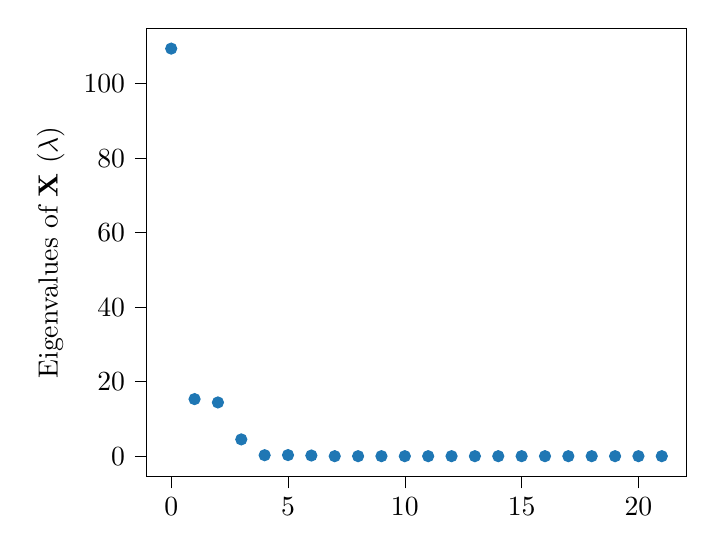
\begin{tikzpicture}

\definecolor{darkgray176}{RGB}{176,176,176}
\definecolor{steelblue31119180}{RGB}{31,119,180}

\begin{axis}[
tick align=outside,
tick pos=left,
x grid style={darkgray176},
xmin=-1.05, xmax=22.05,
xtick style={color=black},
y grid style={darkgray176},
ylabel={Eigenvalues of \(\displaystyle \mathbf{X}\) (\(\displaystyle \lambda\))},
ymin=-5.46944592761344, ymax=114.85836447897,
ytick style={color=black}
]
\addplot [draw=steelblue31119180, fill=steelblue31119180, mark=*, only marks]
table{%
x  y
0 109.388918551398
1 15.3174989008483
2 14.4167178006891
3 4.50008928188145
4 0.259953004649513
5 0.291552925268984
6 0.174200994275395
7 0.00043028047796537
8 0.000426168799885165
9 0.000347654835828332
10 4.94786385683024e-05
11 6.70818529989386e-05
12 6.68982090392825e-05
13 2.28350314823345e-09
14 1.13317580299414e-09
15 9.20035366329261e-10
16 -3.44169916472984e-11
17 -4.14567104661582e-11
18 -3.89423220564401e-11
19 -3.89692406676149e-11
20 -3.89590977559133e-11
21 -3.89603719787611e-11
};
\end{axis}

\end{tikzpicture}
